\documentclass{article}
\usepackage{graphicx}
\begin{document}
	\section*{Lsg Vorschlag LAÜ06 Maximilian Maag}
	\section*{Aufgabe A}
	\begin{itemize}
		\item falsch 
		\item falsch
		\item falsch
		\item falsch
		\item falsch
	\end{itemize}
	\section*{Aufgabe B}
	\subsection*{a)}
	C = $
	\left(\begin{array}{cc}
	-8 & 26 \\  32 & 8
	\end{array}\right)$
	\subsection*{b)}
	C = $
	\left(\begin{array}{ccc}
	10 & 10 & 8 \\ 2 & -26 & 10 \\ 20 & 20 & 16 
	\end{array}\right)$
	\subsection*{c)}
	Inhalt nicht bestimmbar.
	\subsection*{d)}
	C = $
	\left(\begin{array}{ccc}
	-6 & 4 & -2 \\ 22 & 16 & 24
	\end{array}\right)$
	\subsection*{e)}
	C = $
	\left(\begin{array}{ccc}
	17 & 18 & 22 \\ 28 & 29 & 36 \\ 30 & 32 & 39	\end{array}\right)$
	\section*{Aufgabe 1}
	\subsection*{a)}
	2X - 4A = -2B \\
	2X = 4A - 2B \\
	X = 2A - B \\
	X = $
	\left(\begin{array}{ccc}
	-10 & 6 & 8 \\ 8 & 0 & 8
	\end{array}\right)
	$
	\subsection*{b)}
	X + 0,5A = B – 3X \\
	4X = B - 0,5A \\
	X = $\frac{1}{4}$ B - $\frac{1}{8}$ A \\
	X = 
	$\frac{1}{4}$ $\cdot$
	$
	\left(\begin{array}{ccc}
	6 & 2 & -2 \\ 8 & 4 & 0	
	\end{array}\right)$ 
	$
	$
	- $\frac{1}{8}$ $\cdot$
	$
	\left(\begin{array}{ccc}
	-2 & 4 & 2 \\ 8 & 2 & 8	
	\end{array}\right)$ $\cdot$
	$
	$ \\
	X = 
	$
	\left(\begin{array}{ccc}
	\frac{12}{8} & \frac{4}{8} & -\frac{4}{8} \\ 2 & 1 & 0	
	\end{array}\right)$ 
	$
	$
	- 
	$
	\left(\begin{array}{ccc}
	-\frac{2}{8} & \frac{4}{8} & \frac{2}{8}
	 \\ 1 & \frac{2}{8} & 1	
	\end{array}\right)$
	$
	$ \\
	X = 
	$
	\left(\begin{array}{ccc}
	\frac{14}{8} & 0 & -\frac{6}{8} \\ 1 & \frac{8}{8} & -1	
	\end{array}\right)$ 
	$
	$
	\subsection*{c)}
	A – X = 3(B – X) \\
	A – X = 3B – 3X \\
	A + 2X = 3B \\
	2X = 3B - A \\
	X = $\frac{3}{2}$B - $\frac{1}{2}$A \\
	X = $\frac{3}{2}$ $\cdot$
	$
	\left(\begin{array}{ccc}
	 6& 2 &-2 \\ 8& 4& 0
	\end{array}\right)
	$ 
	- $\frac{1}{2}$ $\cdot$
	$
	\left(\begin{array}{ccc}
	-2 & 4 & 2 \\ 8&2 &8 
	\end{array}\right)
	$  \\
	X =
	$
	\left(\begin{array}{ccc}
	\frac{18}{2}& \frac{6}{2} & -\frac{6}{2} \\ \frac{24}{2}& \frac{12}{2}& 0
	\end{array}\right)
	$ 
	- 
	$
	\left(\begin{array}{ccc}
	-\frac{2}{2} & \frac{4}{2} & \frac{2}{2} \\ \frac{8}{2}&\frac{2}{2} &\frac{8}{2} 
	\end{array}\right)
	$  \\
	X =
	$
	\left(\begin{array}{ccc}
	\frac{20}{2}& \frac{2}{2} & -\frac{8}{2} \\ \frac{16}{2}& \frac{10}{2}& -\frac{8}{2}
	\end{array}\right)
	$ \\
	X =
	$
	\left(\begin{array}{ccc}
	10& 1 & -4 \\ 8& 5& -4
	\end{array}\right)
	$ \\
	\section*{Aufgabe 2}
	$	
	\left(\begin{array}{ccc}
	6 & 8 & 4 \\ 5 & 9 & 5 \\ 3 & 12 & 6	\end{array}\right)$ $\cdot$
	$
	\left(\begin{array}{c}
	300 \\ 950 \\ 1750
	\end{array}\right)
	$ = 
	$
	\left(\begin{array}{c}
	16400 \\ 18800 \\ 22800 
	\end{array}\right)
	$ 
	\\ \\
	1. Monat = 16400 € \\
	2. Monat = 18800 € \\
	3. Monat = 22800 €
	
	\section*{Aufgabe 3}
	\subsection*{a)}
	A $\cdot$ P = $
	\left(\begin{array}{ccc}
	1 & 3 & 2 \\ 4 & 6 & 5 \\ 7 & 9 & 8
	\end{array}\right)
	$ \\
	P $\cdot$ A = $
	\left(\begin{array}{ccc}
	1 & 2 & 3 \\ 7 & 8 & 9 \\ 4 & 5 & 6
	\end{array}\right)
	$
	\subsection*{b)}
	Die Multiplikation führt zu diversen Vertauschungen innerhalb der Matrix A.
	\subsection*{c)}
	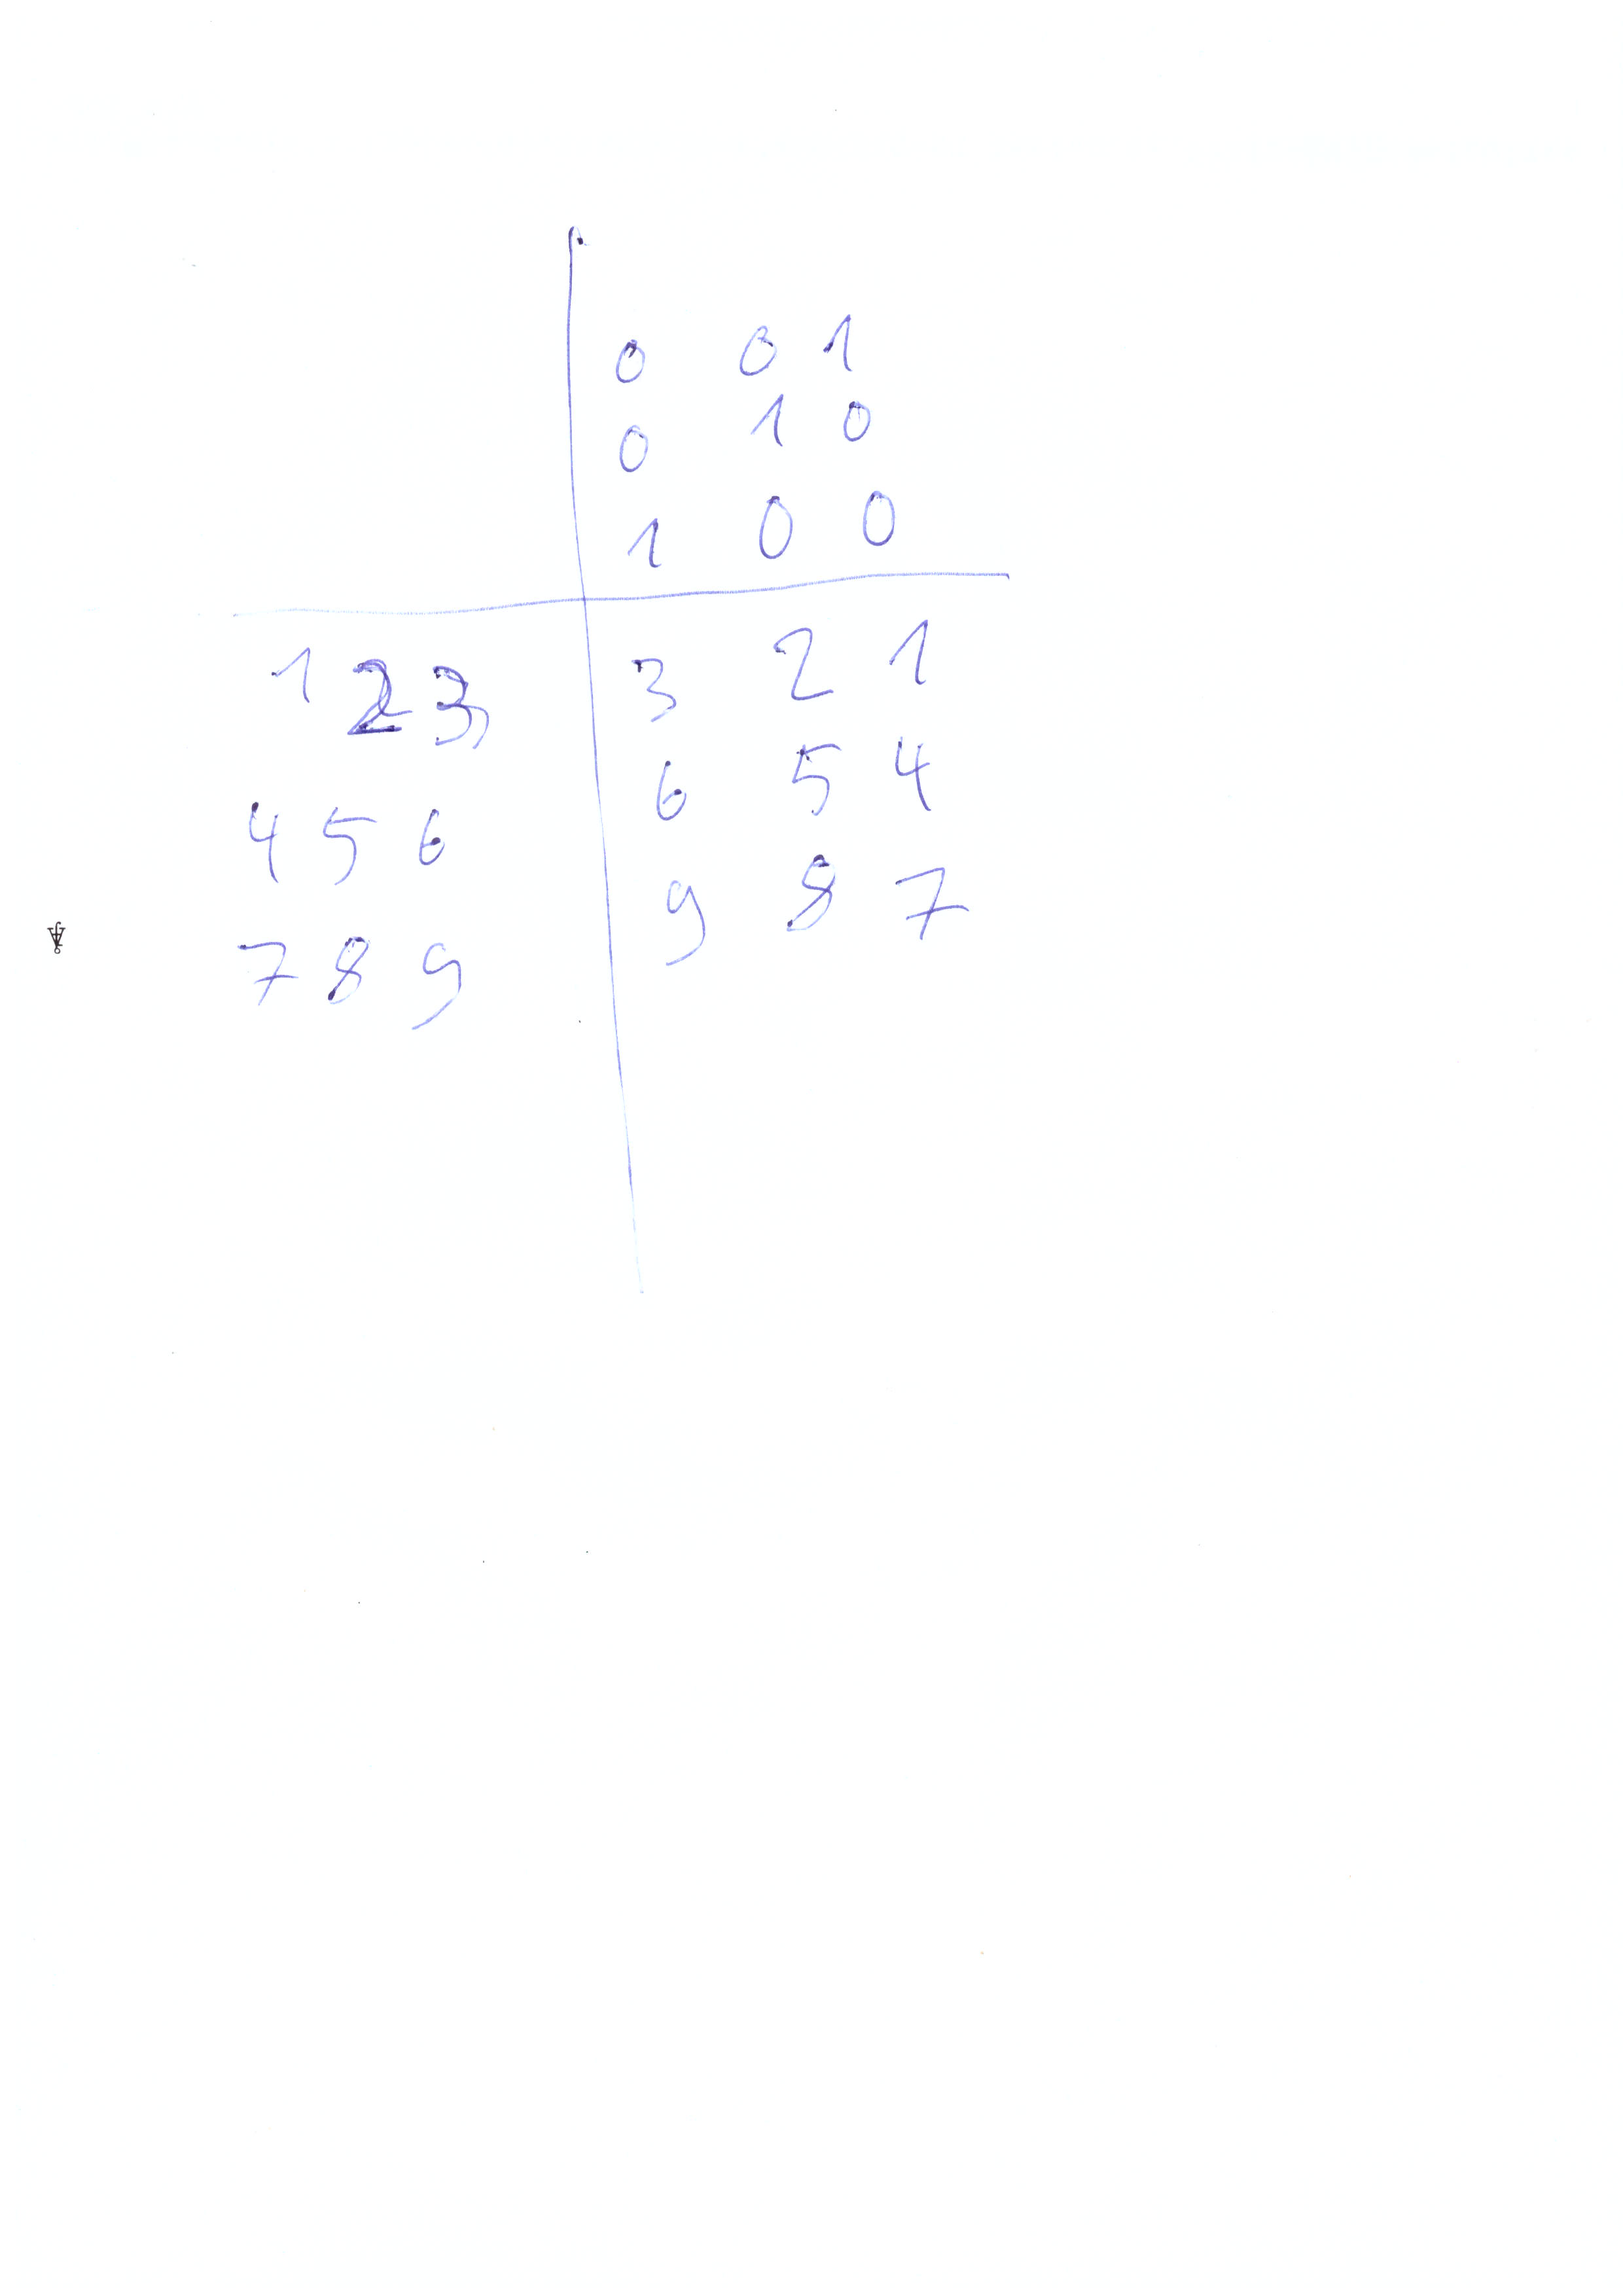
\includegraphics[width=\linewidth]{060301}
	P'  = $
	\left(\begin{array}{ccc}
	 0 & 0 & 1 \\ 0 & 1 & 0 \\ 1 & 0 & 0 
	\end{array}\right)
	$
	\subsection*{d)}
	$\left(
	\begin{array}{ccc}
	1 & 0& 0\\0 &1&0 \\ 0&0&1
	\end{array}
	\right)$
	$\left(
	\begin{array}{ccc}
	0 & 0& 1\\0 &1&0 \\ 1&0&0
	\end{array}
	\right)$
	$\left(
	\begin{array}{ccc}
	0 & 1& 0\\0 &0&1 \\ 1&0&0
	\end{array}
	\right)$
	$\left(
	\begin{array}{ccc}
	1 & 0& 0\\0 &0&1 \\ 0&1&0
	\end{array}
	\right)$
	$\left(
	\begin{array}{ccc}
	0 & 0& 1\\1 &0&0 \\ 0&1&0
	\end{array}
	\right)$
	$\left(
	\begin{array}{ccc}
	0 & 1& 0\\1 &0&0 \\ 0&0&1
	\end{array}
	\right)$ \\ \\
	Bei der Belegung mit Einsen eienr n x n Transformationsmatrix könnte man derart vorgehen, dass man willkürlich in einer Zeile an einer erlaubten Stelle eine 1 setzt. Es ist erlaubt an einer Stelle eine 1 zu setzen sofern in der gleichen Spalte der Zeile keine 1 steht. anschließend setzt man in einer anderen Zeile willkürlich eine 1. Dieser Vorgang muss n-mal wiederholt werden um eine Transformationsmatrix zu erhalten. \\
	n $\cdot$ (n-1) $\cdot$ (n-2) ... $\cdot$ (n-n) \\
	Das entspricht n! Möglichkeiten von n x n Transformationsmatrizen
\end{document}